\section{Make OTB in QGIS Great Again!}

\begin{frame}
\frametitle{2009: OTB-QGIS plugin (Archeology)}
\begin{minipage}[t][6cm][t]{\textwidth}
\begin{center}
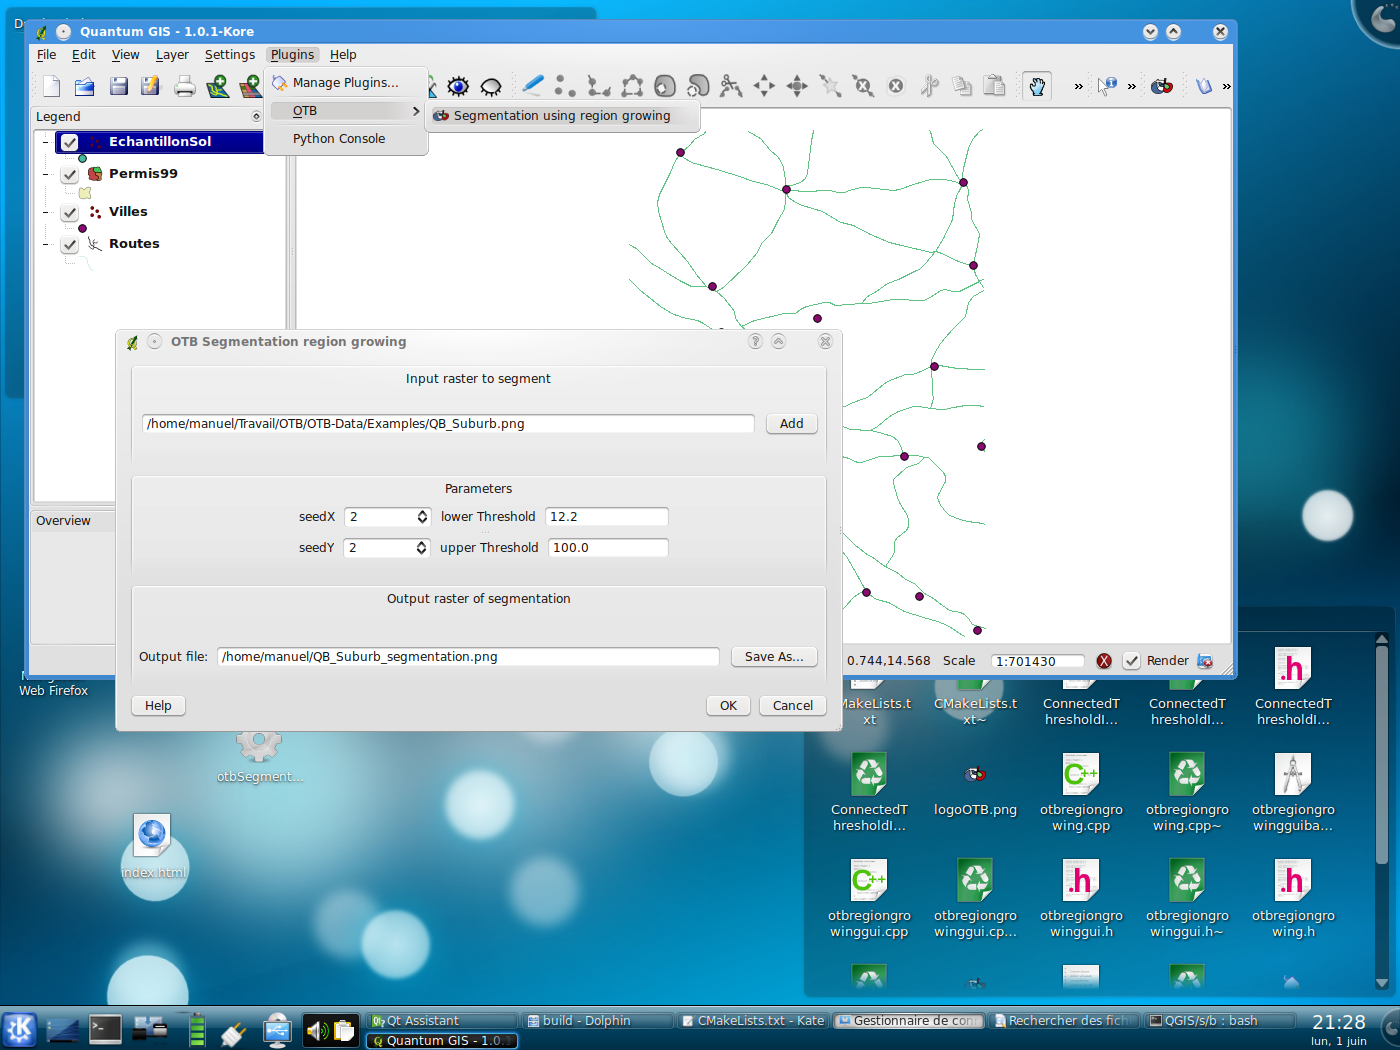
\includegraphics[width=0.7\textwidth]{images/otb-qgis-2009.png}
\end{center}
\end{minipage}
\end{frame}

\begin{frame}
\frametitle{2012-2017: First version of OTB plugin available in QGIS processing}
\begin{minipage}[t][6cm][t]{\textwidth}
\begin{center}
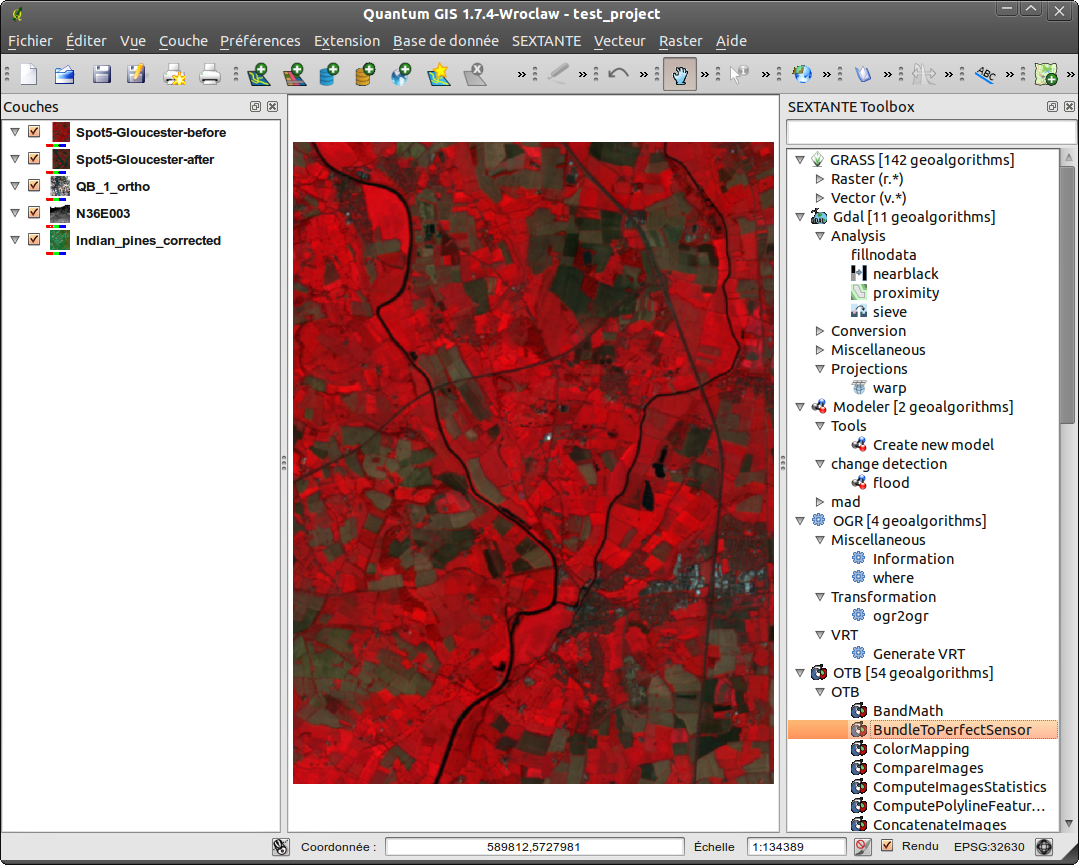
\includegraphics[width=0.7\textwidth]{images/otb_qgis.png}
\end{center}
\end{minipage}
\end{frame}

\begin{frame}
\frametitle{Access to OTB in QGIS: A powerful wedding}
\begin{itemize}
\item Facilitate access to OTB (QGIS widely use in the GIS community)
\item Avoid to duplicate efforts (use QGIS GUI, GIS features...)
\item Powerful features in QGIS processing (batch processing, Python scripting...)
\item Collaboration with the QGIS community is very positive
\item Support from QGIS developers
\item OSGeo \textit{power}
\item \href{https://www.youtube.com/watch?v=ufSQ2SgSIV4}{Demo}: \url{https://www.youtube.com/watch?v=ufSQ2SgSIV4}
\end{itemize}
\end{frame}

\begin{frame}
\frametitle{But everything is not that simple...}
\begin{itemize}
\item ``How to install and configure the last version of OTB in QGIS?''
\item ``Which versions of OTB is compatible with QGIS??''
\item ``Why I can't find the segmentation application in the QGIS processing panel?''
\item ``OTB applications seems to have slightly different names in QGIS?''
\item ``I give up OTB in QGIS...''
\item \alert{STOP!}
\item 2018: We need to improve the integration of OTB in QGIS
%\item Maintenance, Maintenance, Maintenance...
%\item Each version of otb needs to update list of descriptor files
%\item XML files which are hard to maintain.
%\item requires to update a blacklist and whitelist documents to list app that cannot be included and can be included
%\item needs manual update of these xml + followup on pull request
%\item works only with limited version of OTB (Not last release, mostly behind 3-4 releases)
%\item Nobody want to work on it from otb and qgis side. maintained by CS team
%\item Some applications were grouped, depending on their parameters : BinaryMorphologicalOperation (Closing, Dilate, Erode, Opening)
%\item Add new parameter in ParameterMultipleExternalInput processing, to use it in FusionOfClassifications
\end{itemize}

\end{frame}

\begin{frame}
  \frametitle{2018: OTB-QGIS plugin - Age of maturity :)}
  \begin{itemize}
    %\item Easy maintenance for both OTB team and QGIS team
  \item Keep It Simple
  \item Ease the integration of new versions of OTB in QGIS
    %\item Descriptors are generated, distributed and maintained by OTB
  \item Support of OTB binary installers in QGIS (``out of the box'')
  \item All OTB applications available in QGIS (same name, same documentation...)  
    %\item Out of box support for qgis via binary packages
    %\item Applications are not grouped.
    %\item Development took a turn due to some *non-technical*/politic issues in
    %qgis and otb
  \item \alert{Beta version} available as a plugin
  \item Hope the plugin will be soon added to QGIS source code
    %\item Will be added back to QGIS processing core later (Thanks to QGIS team)
    %\item Support for remote modules
    %\item OTB processing provider knows to recreate descriptor file for apps (if not found)
    %\item \alert{Version beta} disponible sous la forme d'un plugin
    % First version is distributed a plugin
  \item
    \href{https://gitlab.orfeo-toolbox.org/orfeotoolbox/qgis-otb-plugin}{https://gitlab.orfeo-toolbox.org/orfeotoolbox/qgis-otb-plugin}{Source
    code of the new plugin}
  \item Compatible with QGIS 3.2
  \item Thanks to all the QGIS team!
  \end{itemize}
\end{frame}

\begin{frame}
\frametitle{OTB configuration in QGIS}
\begin{center}
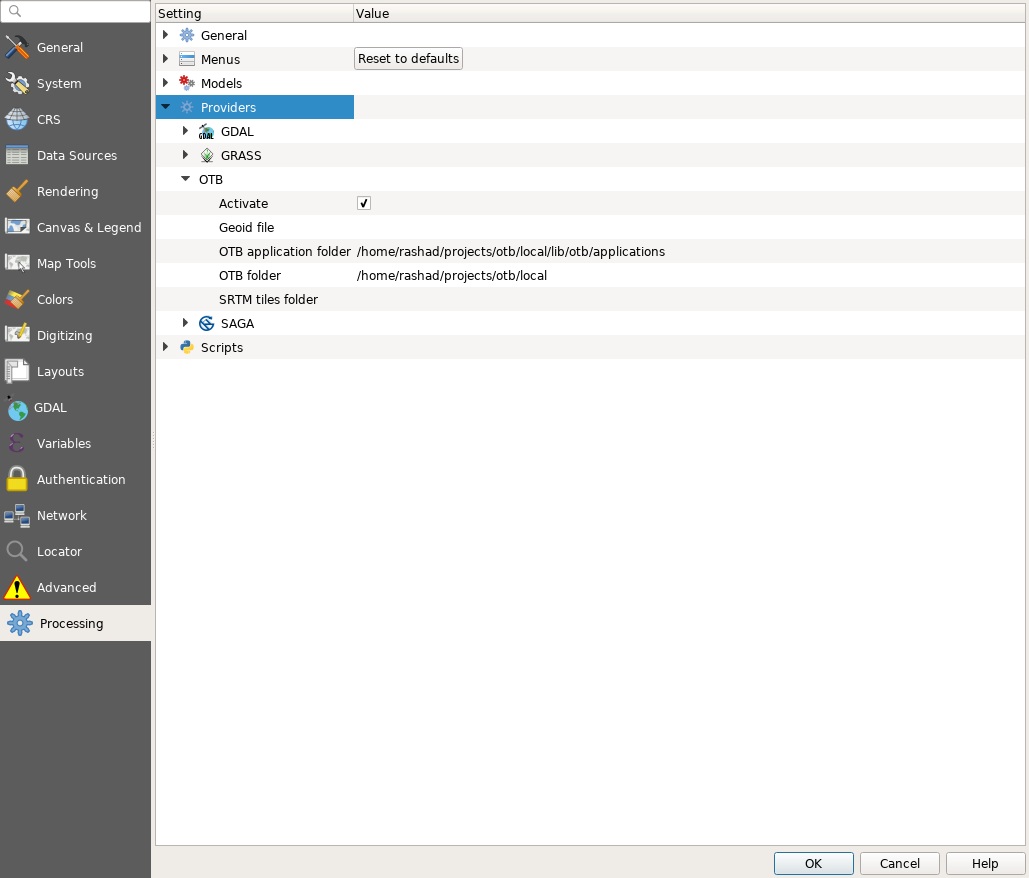
\includegraphics[width=0.8\textwidth]{images/qgis_otb_provider_config.png}
\end{center} 
\end{frame}

\begin{frame}
\frametitle{GUI of the \textit{Smoothing} application}
\begin{center}
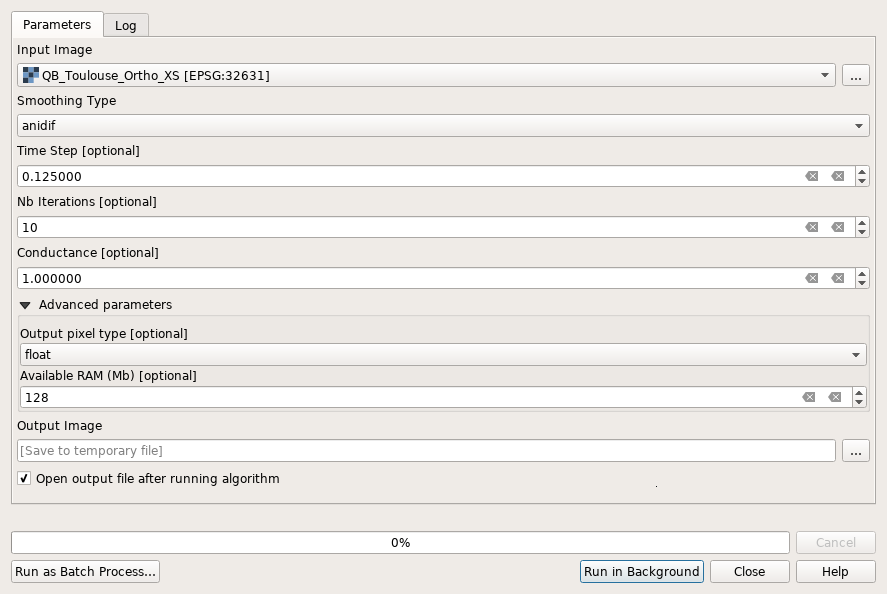
\includegraphics[width=0.8\textwidth]{images/qgis_smoothing.png}
\end{center} 
\end{frame}

\begin{frame}
\frametitle{GUI of the \textit{TrainImagesClassifier} application}
\begin{center}
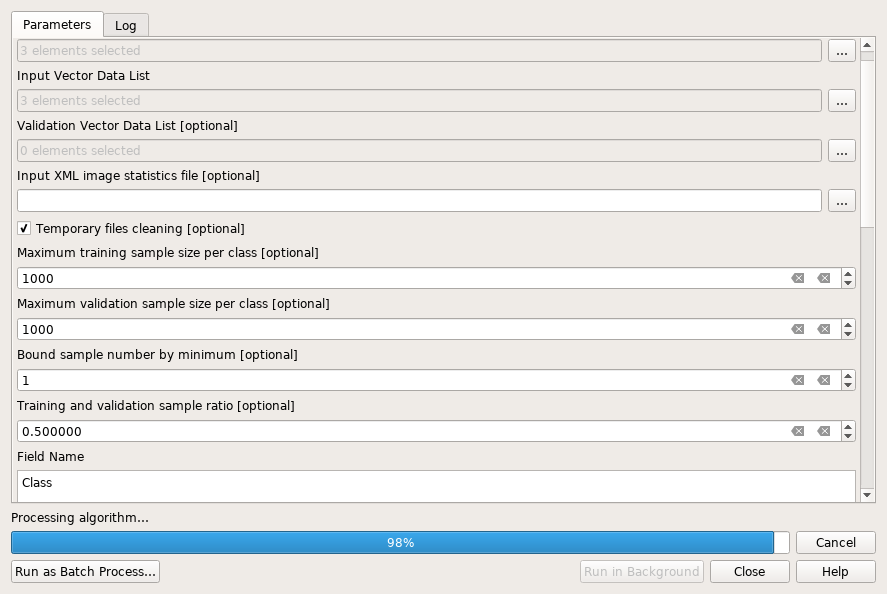
\includegraphics[width=0.8\textwidth]{images/qgis_train_classif.png}
\end{center} 
\end{frame}
